\section{Backlog/roadmap du sprint Beta}

L’objectif de ce sprint est de donner bien plus de valeur à l'utilisateur par:
\begin{enumerate}
    \item Une visualisation des dispositions possible (ce qui apporte bien plus à l'utilisateur que la version Alpha)
    \item Une utilisation facilité par une interface utilisateur intuitive et ergonomique.
\end{enumerate}

Pour ce faire le backlog suivant a été "embarqué" dans cette version et a résulté en la roadmap suivante:


\section{Tests}


\noindent%
\begin{adjustwidth}{-1.5cm}{0cm}

    \renewcommand{\arraystretch}{1.2}
    {\setlength{\tabcolsep}{1.5 mm}

        \begin{testtabular}{|m{0.6cm}|m{5.5cm}|m{8cm}|m{2cm}|c|} \hline
            id                       & Sujet                                                                   & Test d'acceptance                                                                                             & Méthode de test & Résultat \\ \hline
            \multirow{2}{0.6cm}{539} & \multirow{2}{5.5cm}{TACHE Cliquer pour avoir accès aux fonctionnalités} & Quand l'application est lancée, les boutons s'affichent                                                       & Manuel          & OK       \\ \cline{3-5}
            &                                                                         & Quand l'utilisateur clique sur un bouton, la fonctionnalité est activée.                                      & Manuel          & OK       \\ \hline
            \multirow{3}{0.6cm}{538} & \multirow{3}{5.5cm}{TACHE Valider les dimensions}                       & Quand l'application est lancée, seules des valeurs entières peuvent être entrées                              & Manuel          & OK       \\ \cline{3-5}
            &                                                                         & Quand l'application est lancée, les valeurs entrables sont restreintes aux valeurs dans un intervalle défini. & Manuel          & OK       \\ \cline{3-5}
            &                                                                         & Quand l'utilisateur omet ou entre 0 pour au moins une dimension, un message d'erreur s'affiche.               & Manuel          & OK       \\ \hline
        \end{testtabular}}
\end{adjustwidth}


\noindent%
\begin{adjustwidth}{-1.5cm}{0cm}

    \renewcommand{\arraystretch}{1.2}
    {\setlength{\tabcolsep}{1.5 mm}

        \begin{testtabular}{|m{0.6cm}|m{5.5cm}|m{8cm}|m{2cm}|c|} \hline
            id                       & Sujet                                                                                           & Test d'acceptance                                                                                                                                                & Méthode de test & Résultat \\ \hline
            537                      & TACHE Offrir la possibilité d'entrer des dimensions de dojo                                     & Quand l'application est lancée, une fenêtre s'ouvre avec la possibilité d'entrer les dimensions.                                                                 & Manuel          & OK       \\ \hline
            536                      & TACHE Créer la fonction permettant d'afficher toutes les solutions                              & Quand la fonction reçoit en input les coordonnées des tatamis pour une disposition dimensions, alors elle retourne un graph avec toutes les solutions possibles" & Manuel          & OK       \\ \hline
            535                      & TACHE Créer la fonction permettant d'afficher une seule solution                                & Quand la fonction reçoit en input les coordonnées des tatamis pour une disposition dimensions, alors elle retourne un graph avec une solution possible"          & Manuel          & OK       \\ \hline
            534                      & TACHE Créer la fonction permettant de calculer les coordonnées des tatamis pour une disposition & Quand la fonction reçoit en input les dimensions d'un dojo, alors elle retourne les coordonnées des tatamis pour une disposition"                                & Manuel          & OK       \\ \hline
            533                      & TACHE Créer la fonction permettant de choisir d'afficher toutes les solutions                   & Étant donné les inputs des dimensions d'un dojo, quand cette fonction est choisie, elle retourne un graph avec toutes les solutions possibles"                   & Manuel          & OK       \\ \hline
            532                      & US Disposer d'une interface d'affichage ergonomique                                             & Quand le programme est lancé, il ouvre une interface ergonomique"                                                                                                & Manuel          & OK       \\ \hline
            531                      & TACHE Créer une classe de fenêtre type permettant d'avoir un affichage reproductible            & Quand l'application est lancée, une fenêtre s'ouvre avec les bonnes (adaptées à l'écran) et memes dimensions"                                                    & Manuel          & OK       \\ \hline
            530                      & TACHE Créer la fonction permettant de choisir d'afficher une seule solution                     & Étant donné les inputs des dimensions d'un dojo, quand cette fonction est choisie, elle retourne un graph avec une seule solution possible"                      & Manuel          & OK       \\ \hline
            \multirow{2}{0.6cm}{519} & \multirow{2}{5.5cm}{EPIC Permettre au gestionnaire de dojo de visualiser les solutions}         & cf. tests utilisateurs des US                                                                                                                                    &                 & OK       \\ \cline{3-5}
            &                                                                                                 & Le nombre de solution du programme donne le meme nombre de solution que le calcul de coordonnées Tatamis                                                         & Automatisé      & OK       \\ \hline
            478                      & US Afficher visuellement toutes les dispositions possibles                                      & Étant donné des dimensions d'un dojo saisies, quand il sélectionne cette option, il obtient visuellement toutes les dispositions possibles"                      & Manuel          & OK       \\ \hline
            476                      & US Afficher visuellement une disposition possible                                               & Étant donné des dimensions d'un dojo saisies, quand il sélectionne cette option, il obtient visuellement une disposition possible"                               & Manuel          & OK       \\ \hline
        \end{testtabular}
    }
\end{adjustwidth}

\bigskip

Les tests automatisés sont définis dans le fichier \texttt{testbeta.py}. Ils peuvent être reproduits en l'exécutant avec ligne de commande 
\texttt{python3 -m pytest}.

\section{Documentation utilisateur Beta}

\subsection{Prérequis}

Configuration et installations requises:
\begin{itemize}
    \item Python 3.9 ou supérieur
    \item Librairies Python: datetime, numpy, PyQt5.QtCore, PyQt5.QtGui, PyQt5.QtWidgets, sys, time.
\end{itemize}


\subsection{Comment trouver le nombre de tatamis nécessaires pour remplir un dojo?}

\begin{enumerate}
    \item Lancer l’interface (dans le Terminal avec la ligne de commande: \texttt{python3 interface.py})
    \item Entrer dans l’interface la longueur et la largeur du dojo dans les champs prévus à cet effet.

          \emph{Nb:
              \begin{itemize}
                  \item Vous pouvez inverser la longueur et la largeur, cela n’a pas d’importance
                  \item Vous pouvez entrer un nombre de tatamis compris entre 1 et 25.
              \end{itemize}
          }
    \item Cliquer sur le bouton: “Connaître le nombre de tatamis 2x1 nécessaires pour la taille du dojo”
          \emph{ Nb: Si vous oubliez d’entrer une dimension ou si vous entrez une dimension 0,
              un message d’erreur “Erreur de saisie des dimensions. Aucune dimension ne peut avoir une valeur nulle ou vide” apparaît.}
    \item Interpréter la réponse:
          \begin{enumerate}
              \item  \textbf{Réponse}: “Le nombre de tatamis 2x1 nécessaires pour ce dojo est : [Nombre]”.
                    \textbf{Interprétation}: il existe au moins une disposition possible et vous aurez besoin d’exactement [Nombre] tatamis pour remplir le dojo.
              \item  \textbf{Réponse}: “Le nombre de tatamis 2x1 nécessaires pour ce dojo est :
                    Aucune disposition possible de tatamis 2x1 pour ce dojo”. \textbf{Interprétation}:
                    il n’existe aucune disposition possible de tatamis 2 x 1 pour remplir le dojo.
          \end{enumerate}
\end{enumerate}

\subsection{Comment savoir s’il existe une disposition possible de tatamis pour un dojo donné?}

\begin{enumerate}
    \item Lancer l’interface (dans le Terminal avec la ligne de commande: \texttt{python3 interface.py})
    \item Entrer dans l’interface la longueur et la largeur du dojo dans les champs prévus à cet effet.

          \emph{Nb:
              \begin{itemize}
                  \item Vous pouvez inverser la longueur et la largeur, cela n’a pas d’importance
                  \item Vous pouvez entrer un nombre de tatamis compris entre 1 et 25.
              \end{itemize}
          }
    \item Cliquer sur le bouton: “Savoir s’il existe une disposition pour le dojo”

          \emph{Nb: Si vous oubliez d’entrer une dimension ou si vous entrez une dimension 0,
              un message d’erreur “Erreur de saisie des dimensions.
              Aucune dimension ne peut avoir une valeur nulle ou vide” apparaît.}
    \item Interpréter la réponse:
          \begin{enumerate}
              \item \textbf{Réponse}: “Il existe au moins une disposition avec des tatamis 2x1 pour ce dojo”.
                    \textbf{Interprétation}: il existe au moins une disposition possible.
              \item \textbf{Réponse}: “Il n’existe pas de disposition possible avec des tatamis 2x1 pour ce dojo”.
                    \textbf{Interprétation}: il n’existe aucune disposition possible de tatamis 2 x 1 pour remplir le dojo.
                    Il est dans ce cas probable de devoir utiliser des demi-tatamis pour remplir pleinement le dojo.
          \end{enumerate}

\end{enumerate}

\subsection{Comment savoir combien il existe des dispositions possibles de tatamis pour un dojo donné?}

\begin{enumerate}
    \item Lancer l’interface (dans le Terminal avec la ligne de commande: \texttt{python3 interface.py})
    \item Entrer dans l’interface la longueur et la largeur du dojo dans les champs prévus à cet effet.

          \emph{Nb:
              \begin{itemize}
                  \item Vous pouvez inverser la longueur et la largeur, cela n’a pas d’importance
                  \item Vous pouvez entrer un nombre de tatamis compris entre 1 et 25.
              \end{itemize}
          }
    \item Cliquer sur le bouton: “Connaître le nombre dispositions possibles”.

          \emph{Nb: Si vous oubliez d’entrer une dimension ou si vous entrez une dimension 0,
              un message d’erreur “Erreur de saisie des dimensions.
              Aucune dimension ne peut avoir une valeur nulle ou vide” apparaît.
          }
    \item Interpréter la réponse:
          \begin{enumerate}
              \item \textbf{Réponse}: “Il existe [Nombre] dispositions possibles”.
                    \textbf{Interprétation} : il existe des dispositions pour ce dojo et [Nombre] est
                    le nombre de dispositions possibles pour remplir le dojo.
              \item \textbf{Réponse}: “Il existe 0 disposition possible”.
                    \textbf{Interprétation}: la demande est non pertinente car il n’existe pas de disposition possible
                    de tatamis 2x1 pour les dimensions du dojo.
          \end{enumerate}
\end{enumerate}


\subsection{Comment afficher une disposition?}

\begin{enumerate}
    \item Lancer l’interface (dans le Terminal avec la ligne de commande: \texttt{python3 interface.py})
    \item Entrer dans l’interface la longueur et la largeur du dojo dans les champs prévus à cet effet.

          \emph{Nb:
              \begin{itemize}
                  \item Vous pouvez inverser la longueur et la largeur, cela n’a pas d’importance
                  \item Vous pouvez entrer un nombre de tatamis compris entre 1 et 25.
              \end{itemize}
          }
    \item Cliquer sur le bouton: “Afficher une disposition”

          \emph{Nb: Si vous oubliez d’entrer une dimension ou si vous entrez une dimension 0,
              un message d’erreur “Erreur de saisie des dimensions.
              Aucune dimension ne peut avoir une valeur nulle ou vide” apparaît.
          }

    \item Une disposition s’affiche

          Ou bien le message d’erreur suivant s’affiche: “Demande impossible.
          Il n'existe pas de disposition possible avec des tatamis 2x1 pour ce dojo” apparaît,
          ce qui signifie que la demande est non pertinente car il n’existe pas de disposition
          possible de tatamis 2x1 pour les dimensions du dojo.

\end{enumerate}

\subsection{Comment afficher toutes les dispositions possibles?}


\begin{enumerate}
    \item Lancer l’interface (dans le Terminal avec la ligne de commande: \texttt{python3 interface.py})
    \item Entrer dans l’interface la longueur et la largeur du dojo dans les champs prévus à cet effet.

          \emph{Nb:
              \begin{itemize}
                  \item Vous pouvez inverser la longueur et la largeur, cela n’a pas d’importance
                  \item Vous pouvez entrer un nombre de tatamis compris entre 1 et 25.
              \end{itemize}
          }
    \item Cliquer sur le bouton: “Afficher toutes les dispositions possibles”

          \emph{Nb: Si vous oubliez d’entrer une dimension ou si vous entrez une dimension 0,
              un message d’erreur “Erreur de saisie des dimensions.
              Aucune dimension ne peut avoir une valeur nulle ou vide” apparaît.
          }

    \item Toutes les dispositions possibles s’affichent

          Ou bien le message d’erreur suivant s’affiche: “Demande impossible.
          Il n'existe pas de disposition possible avec des tatamis 2x1 pour ce dojo” apparaît,
          ce qui signifie que la demande est non pertinente car il n’existe pas de disposition
          possible de tatamis 2x1 pour les dimensions du dojo.

\end{enumerate}

\section{Explication des algorithmes et choix de programmation}

\subsection{Algorithme pour l’affichage des dispositions}

\subsubsection{Première solution envisagée}

La première solution envisagée afin d’afficher la disposition des tatamis comprenait l’utilisation
de la bibliothèque python facile, dont une application au pavage de surface par tatamis a été trouvée
sur le site de Xavier Olive\footnote{https://www.xoolive.org/2016/02/29/pavage-par-tatamis.html}.  La publication semblait correspondre exactement à ce que nous souhaitions,
à savoir un calcul des dispositions possibles, et un affichage graphique adapté (via la bibliothèque matplotlib ).

La bibliothèque facile permet de modéliser et résoudre un problème en programmant ses contraintes.
Les positions et les directions des tatamis constituent les variables du problème.

Les contraintes étant constituées par les assertions suivantes:

\begin{itemize}
    \item deux tatamis ne peuvent pas se chevaucher
    \item les tatamis ne sortent pas du cadre
    \item quatre tatamis ne peuvent pas se rejoindre en un point
\end{itemize}

L’utilisation des algorithmes proposés comportait néanmoins plusieurs inconvénients :

\begin{itemize}
    \item Un temps de calcul devenant rapidement bloquant pour des dimensions de dojo encore raisonnables (16 $\times$ 16).
    \item Une bibliothèque complexe à appréhender, elle-même issue d’une adaptation en python
          de fonctionnalités développées en OCaml.
\end{itemize}

Nous aurions pu nous contenter de cette solution, mais l’impossibilité d’obtenir des pavages
pour des dimensions au-delà de 16 $\times$ 16 nous a semblé rédhibitoire.

\subsubsection{Solution retenue}

Après une recherche un peu plus poussée, il s'est avéré que ce problème de pavage dit "tatamis-parfait"
fait l'objet d'une question dans un livre édité en chinois et dont la traduction anglaise proposée pour le titre
est : "Programmer's algorithm interesting topic". Les problèmes traités dans ce livre le sont initialement en Ruby et Javascript,
néanmoins un internaute chinois propose une interprétation de l'algorithme en python sur une note de
blog\footnote{https://blog.csdn.net/chenxy\_bwave/article/details/120364982}\label{chenxy}.
Celle-ci ayant été traduite en anglais\footnote{https://www.fatalerrors.org/a/programmer-s-algorithm-interesting-topic-q32-laying-method-of-tatami.html},
nous avons pu en prendre plus facilement connaissance et ainsi en exploiter les idées.\\

L'auteur de cette note propose de modéliser la pièce en la découpant selon une grille d'intervalle 1.\\

Le problème est identifié comme celui d'un parcours de graphe (arbre binaire) en profondeur d'abord.
La racine de l'arbre étant constituée par une pièce vide de tatami. Chaque nœud du graphe correspond
à un état de pavage donné, où chaque zone de la grille contient un entier correspondant au numéro du
tatami qui la recouvre. Le nombre 0 désigne alors une zone vide de tatami.\\

La pièce est donc modélisée par une matrice de dimension H*W où H désigne sa hauteur et W sa largeur.
Afin de détecter les bords de la pièce lors du parcours, la matrice est “bordée” par le nombre -1.\\

Le cœur du problème consiste à savoir si une zone de la grille peut être recouverte par un tatami.
Étant donné que nous ne voulons pas que quatre tatamis se rejoignent en même coin, le critère est donc
qu’une zone ne peut être pavée que si les trois positions de la grille situées à gauche, en haut à gauche,
et en haut ne sont pas toutes pavées par des tatamis différents.
Cette situation est traduite par l’illustration ci-dessous :\\

\begin{center}
    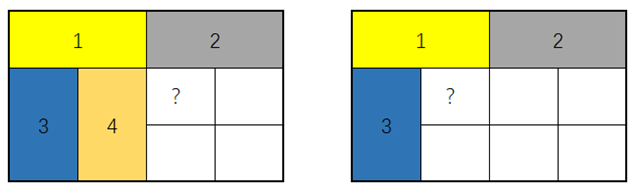
\includegraphics[width=10cm]{images/illustrationBeta-algo-2.png}
\end{center}

L’algorithme parcourt la grille ligne par ligne et colonne par colonne en vérifiant pour chaque position
si un tatamis peut-être posé : dans un premier temps en position horizontale, puis dans un deuxième temps
en position verticale. Si c’est le cas, la position de la grille ainsi que sa zone adjacente (horizontale ou verticale)
reçoivent le numéro du tatami courant et l’algorithme est appelé pour la position suivante, en incrémentant le numéro du tatami.
Lorsque la ligne atteinte correspond au bord bas du tatamis, le pavage est complet.\\

L’auteur précise qu’un tel parcours peut comporter une profondeur considérable selon les dimensions de la pièce
à paver et que selon les cas on peut donc atteindre rapidement la profondeur de récursivité maximale.\\

L'illustration d'un parcours de recherche pour un pavage (4$\times$3) est donnée ci-dessous.\\

\begin{adjustwidth}{-1.5cm}{0cm}
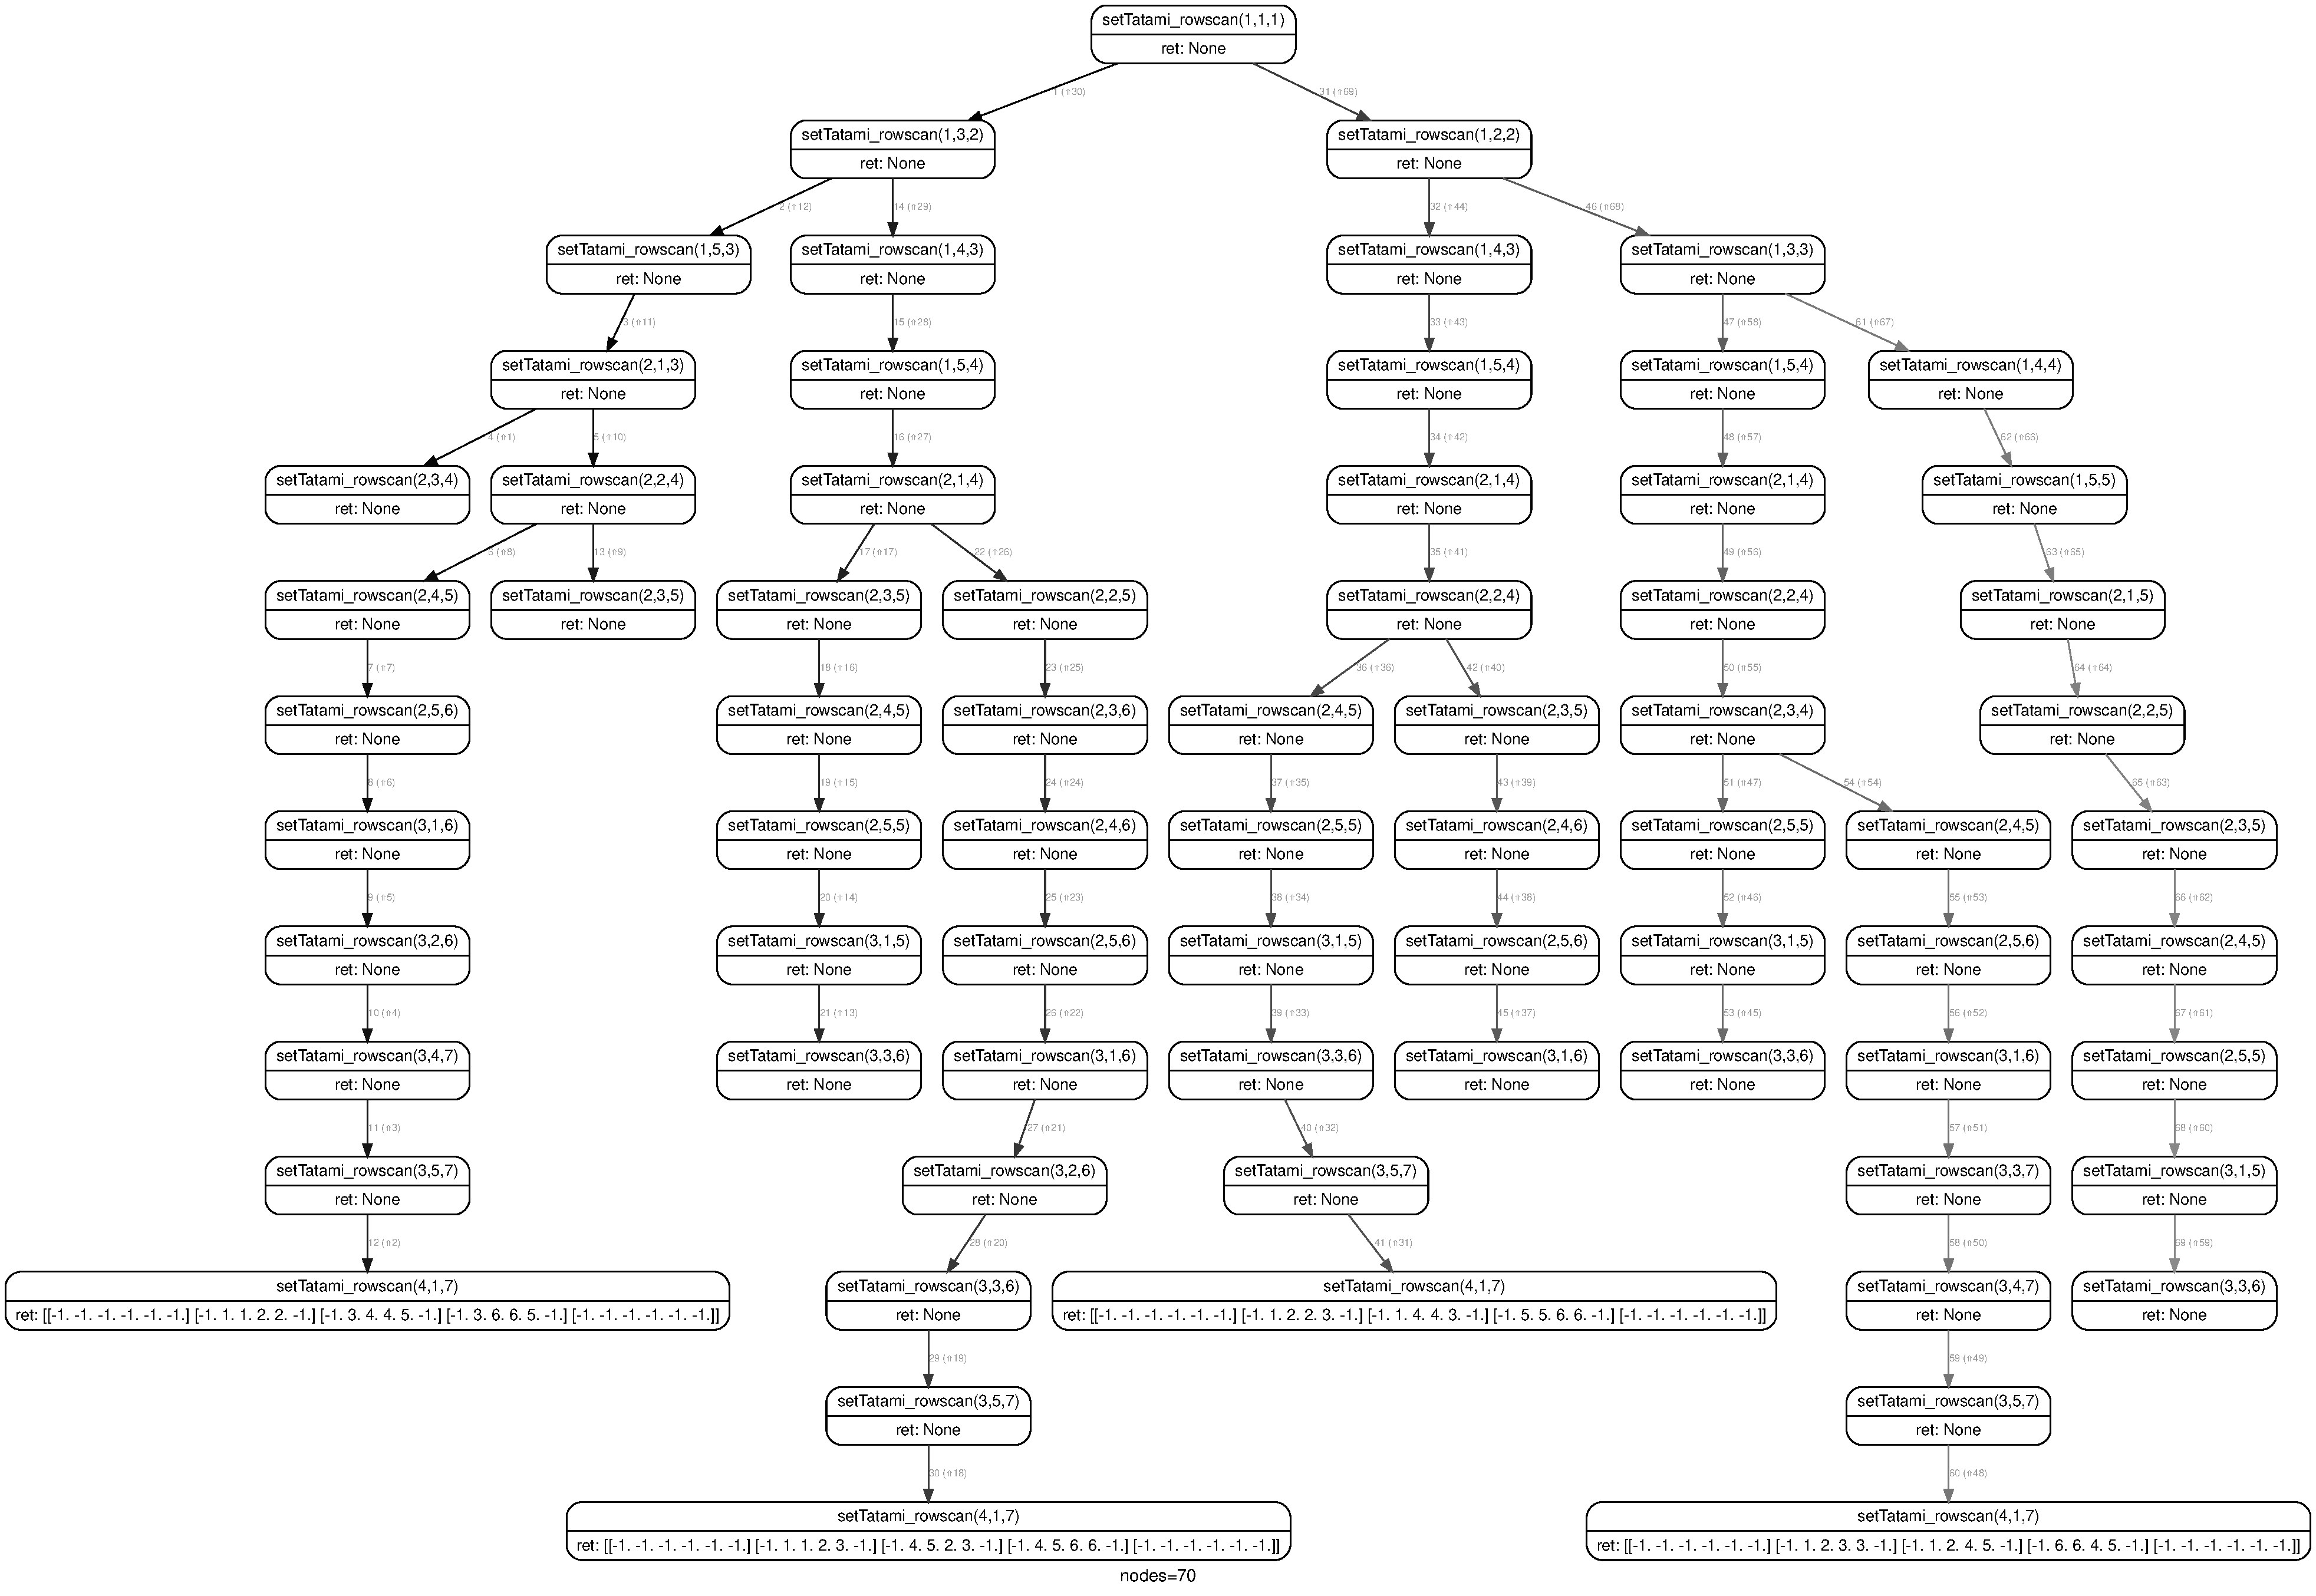
\includegraphics[width=19cm]{images/arbre4x3.pdf}
\end{adjustwidth}


En testant le programme en Python proposé par l’auteur, nous atteignons effectivement une limite de calcul,
mais celle-ci nous permet néanmoins de traiter des dojos plus grands que la solution évoquée précédemment.
Nous augmentons ainsi notre capacité de traitement d’environ 80\% puisque la dimension limite de dojo passe de 16 à 25.\\

La publication originale fournissait l’implémentation d’une fonction récursive manipulant des variables globales.
Afin de pouvoir utiliser cette solution dans notre projet, la fonction a été intégrée au sein d’une classe en tant que méthode,
et les variables globales sont devenues des attributs de celle-ci. La fonction initiale ne retournant qu’une matrice d’index,
il a fallu ajouter une méthode de classe afin de produire à partir de cette matrice, les positions de chaque tatami dans le plan.
L’enregistrement des positions se faisant à l’aide d’une liste de dictionnaire, chacun de ces dictionnaires contenant
les caractéristiques d’un tatami (index, largeur, longueur, position verticale et position horizontale).



\subsection{Choix de programmation Interface}

Les choix importants concernant l’interface ont été les suivants:


\subsubsection{Choix de la librairie d’interface graphique}

Une recherche initiale a permis d'identifier 5 librairies à notre disposition:

\begin{itemize}
    \item PyQt5
    \item Tkinter
    \item Pyside2
    \item Kivy
    \item wxPython
\end{itemize}

Trois critères de choix ont été appliqués:

\begin{itemize}
    \item Capacités de la librairie
    \item Disponibilité de la documentation et ressources en ligne
    \item Connaissances préalables par l'équipe et simplicité
\end{itemize}

L'évaluation a conclu aux résultats suivants:\\


\noindent%
\begin{adjustwidth}{-1.5cm}{0cm}

    \renewcommand{\arraystretch}{1.2}
    {\setlength{\tabcolsep}{1.5 mm}


        \begin{testtabular}{*{6}{|p{0.16\linewidth} }|} \hline

            \rowcolor{tsgrey}                               &                                                                                                & Tkinter & Pyside2 & Kivy & wxPython \\ \hline
            \cellcolor{lightgray} Capacités de la librairie & Très large variété de widgets (boutons, champs de saisie, boîtes de message…)

            Beaucoup de possibilités

            Grille disponible
            & Large variété de widgets (boutons, champs de saisie, boîtes de message…)

            Grille disponible (mais également une fonctionnalité qui facilite le placement)
            & Large variété de widgets (boutons, champs de saisie, boîtes de message…)

            Grille disponible
            & Widgets disponibles, dont certains bien designés mais d’autres moins intuitifs (par ex. les boutons)

            Grille disponible
            & Large variété de widgets (boutons, champs de saisie, boîtes de message…)

            Grille disponible
            \\ \hline

            \cellcolor{lightgray} Disponibilité de la documentation et ressources en ligne & 20 000 questions sur Stackoverflow

            & 45 000 questions sur Stackoverflow
            & 1 500 questions sur Stackoverflow
            & 12 000 questions sur Stackoverflow
            & 7 000 questions sur Stackoverflow
            \\ \hline

            \cellcolor{lightgray} Connaissances préalables et simplicité & Connaissances préalables de l'équipe & Peu de connaissances
            Mais facile a comprendre
            & Non & Non  & Non
            \\ \hline



        \end{testtabular}

    }
    % compléter tableau : disponibilité de la doc & connaissances préalables
\end{adjustwidth}

\bigskip

Compte tenu de cette évaluation, le choix entre PyQt5 et Tkinter n’a pas été évident.
Étant donné les connaissances préalables de l'équipe en PyQt5 et les possibilités plus importantes
de la librairie par rapport à Tkinter, c’est PyQt5 qui a finalement été choisi.

\subsubsection{Choix concernant la disposition des éléments de l’interface}

Deux options ont été étudiées:
Positionnement spécifique de chaque élément de l’interface (par la fonction \texttt{move()} de PyQt5)
Avantage:    Flexibilité (possibilité de placer très précisément chaque objet sur les axes abscisse et ordonnées de la fenêtre)
Inconvenient:    Fastidieux (nécessite de placer chaque objet avec ses coordonnées et les modifications de disposition - notamment par l’ajout d’objet - s’en trouve très longs à exécuter)
Positionnement par la mise en place et utilisation d’une grille (invisible à l'utilisateur) pour placer les éléments (par la sous-librairie QGridLayout de PyQt5)
Avantages:    Rapidité à coder (possibilité de placer très précisément chaque objet sur les axes abscisse et ordonnées de la fenêtre)
Bon alignement obtenu très facilement obtenu (car la grille assure le bon alignement)
Inconvenient:    Moins de flexibilité pour placer précisément les objets

Étant donné les avantages importants de l’option 2 et le fait que l’interface pour notre programme pouvait facilement être mise en place sous forme d’une grille, l’option 2 a été choisie.


\subsubsection{Choix concernant l’intuitivité de l’interface}

Pour cette première 'vraie' interface pour l’utilisateur
(sachant qu’en version Alpha, l’utilisateur interagissait avec le programme par l'intermédiaire du Terminal),
des choix importants et engageants pour la suite ont été à faire. De manière générale,
il a été choisi de mettre un focus particulier sur la facilité d’utilisation et l’intuitivité pour l’utilisateur.
Pour ce faire voilà les principales questions qui ont été étudiées et  choix effectués:

\begin{enumerate}
    \item Appel des fonctionnalités

          Pour une utilisation facile et compréhension des fonctionnalité disponible, il a été choisi
          d'utiliser des boutons pour l’appel des fonctionnalités, et de laisser beaucoup d’espace
          dans le boutons pour y afficher les fonctionnalité en détails
    \item Manière d’exprimer les retours

          Pour une qualité d’utilisation, tous les retours (message d’erreur ou réponse attendue par l’utilisateur)
          sont exprimés par des fenêtres "pop up"
    \item Guidance d’utilisation, "formation" des utilisateurs et information

          Il a été choisi de mettre un focus particulier sur ces aspects pour fournir une grande qualité de programme.
          L’objectif est de guider au maximum l’utilisateur (pour "borner" ses actions à ce qui est autorisé) et
          de fournir des messages de retour clairs pour chaque type d’erreur ou d'impossibilité d’utilisation de fonctionnalités.
          Voici les principales mesures mises en place :
          \begin{itemize}
              \item Les champs de saisie sont extrêmement guidés par une validation (à l'aide de la fonction \texttt{QIntValidator}):
                    l’utilisateur ne peut saisir que des entiers entre les valeurs inscrites sur l’interface
              \item Les seules saisies impossibles à contrôler sont la saisie de "0" ou l’absence de saisie, mais des messages d’erreur
                    ont été mis en place.
              \item Des tests sont effectués avant l’appel de chaque fonctionnalité pour savoir si la fonctionnalité est disponible avec
                    les dimensions de dojo saisies. Dans le cas contraire, un message d’erreur clair est donné à l'utilisateur.
              \item Tous les cas d’erreurs ont été traités (un utilisateur ne peut pas se retrouver bloqué en produisant une erreur
                    qui ne retourne pas une explication sur comment la résoudre)
          \end{itemize}

\end{enumerate}


\subsubsection*{Interface et messages de retour:}


\begin{itemize}
     

    \item Interface :

\begin{center}
    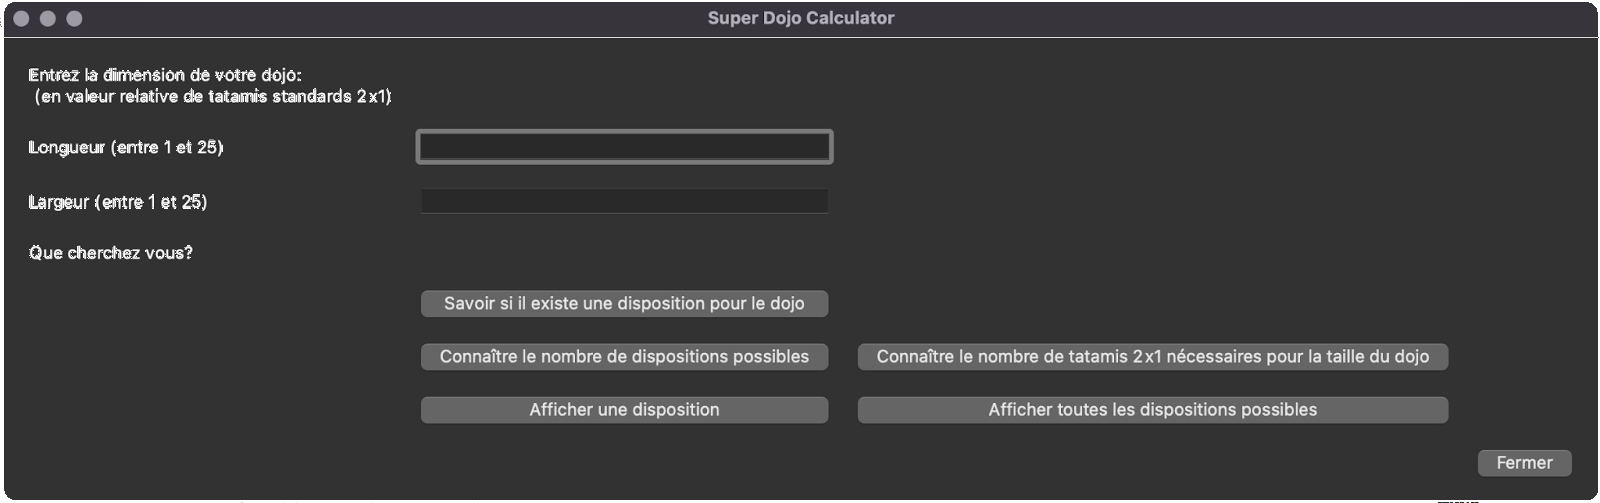
\includegraphics[scale=0.25]{images/betaInterface.png}
\end{center}


\item Exemple de message de retour (succès):

\begin{center}
    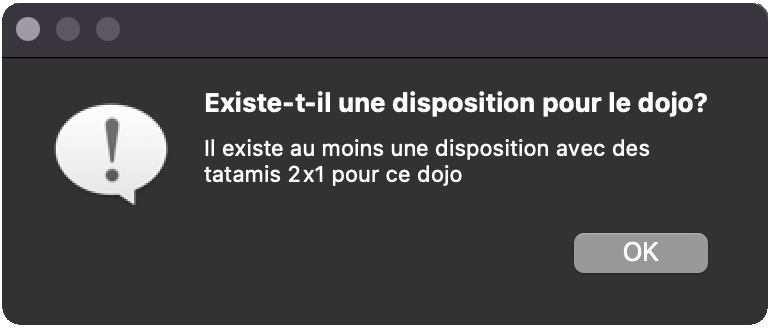
\includegraphics[scale=0.25]{images/betaRetourSucces.png}
\end{center}


\item Exemple de message indiquant à l’utilisateur que la demande est impossible avec les dimensions saisies:

\begin{center}
    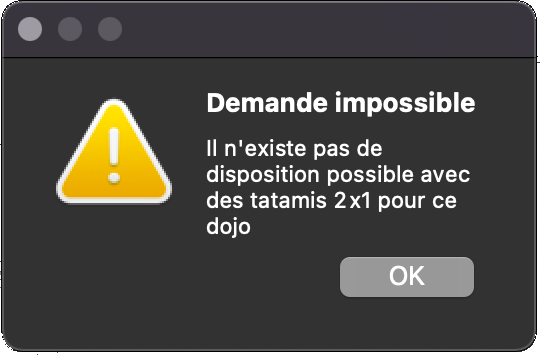
\includegraphics[scale=0.25]{images/betaImpossible.png}
\end{center}


\item Exemple de message d’erreur en cas de non saisie ou saisie nulle de dimensions:

\begin{center}
    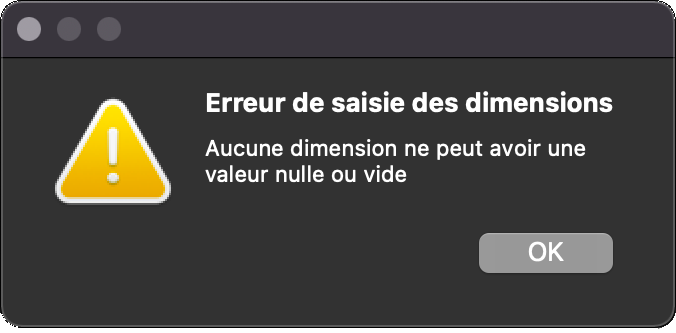
\includegraphics[scale=0.25]{images/betaErreurSaisie.png}
\end{center}


\end{itemize}

\subsection{Choix de la structure du programme}

Dans la continuité des choix fait en version Alpha, nous avons mis en application des principes \emph{SOLID}, et en particulier du
\emph{Single Responsibility Principle} et \emph{Open-Closed Principle}:

\begin{itemize}
    \item Un fichier a une fonction principale
          Dans cette version beta, nous sommes passés de 2 fichiers (un fichier de front-end \texttt{interface.py} et un fichier de back-end \texttt{alpha.py}) à
          4 fichiers du fait de la croissance des fonctionnalités et des besoins de calculs en back-end. Nous avons donc:
          \begin{itemize}
              \item \texttt{interface.py}: fichier qui continue à contenir toutes les fonctionnalités de front-end, c’est à dire l’interface utilisateur
              \item \texttt{calcul\_coordonnees\_tatamis.py}: classe qui calcule les coordonnées des tatamis d'après les dimensions du dojo.
                    Cette classe contient la fonction permettant de calculer une solution de pavage, d’après le code trouvé sur la publication
                    citée dans la partie \ref{chenxy}, à laquelle a été adjointe une fonction permettant d’obtenir les coordonnées des tatamis dans le plan.
              \item \texttt{calcul\_nombre\_dispositions.py}: fichier qui reprend les fonctions de calculs (basiques) de back-end de la version alpha.
              \item \texttt{dojo.py} : classe permettant d'instancier un tatamis d'après ces propriétés: position, dimensions, couleur. L’affichage
                    des solutions graphiques se faisant dans une fenêtre à part et utilisant des fonctions particulières, cela justifiait
                    l’existence d’une classe spécifique.
          \end{itemize}
    \item Chaque fonction a un seul usage. Plusieurs exemples peuvent être cités dans le fichier \texttt{interface.py}: de nombreuses
          fonctions à fonctionnalité très limitée mais réutilisables ont été créées comme par exemple \texttt{set\_longueur()}, \texttt{set\_largeur()}, 
          \texttt{valeur\_vide(self)}, \texttt{clickExiste()} (leur fonctionnalité est documentée dans le code et donc non-reprise dans ce rapport)

    \item Dans la mesure du possible des fonctions ou classes génériques sont créées puis réutilisées.
          Un bon exemple a cela sont les classes génériques de l’interface: \texttt{MessageSaisieInvalide}, \texttt{MessageDemandeImpossible} et \texttt{MessageInfo}.
\end{itemize}



\section{Challenges rencontrés et apprentissage}

\subsection{Challenges rencontrés et solutions appliquées}

Les deux challenges principaux de cette version ont été les suivants:
\begin{enumerate}
    \item Challenges techniques
    
          Comme on peut le constater plus dans la section sur les choix de programmation, il s’agit de la version la plus complexe techniquement.
          D’un point de vue de l’algorithme, l’affichage des dispositions a été un gros challenge technique.
          D’un point de vue de l’interface, beaucoup de choix structurants ont été nécessaires, avec des essais et révisions.
          Enfin, d’un point de vue de l’architecture du programme, les choix faits en version Alpha ont été à implémenter de manière plus poussée.
          Pour faire face à ces challenges, nous avons adopté l’approche suivante:
          \begin{itemize}
              \item Planification en systématiquement décomposant les "gros" problèmes en problèmes plus petits
              \item Recherches techniques avant tout choix à faire
              \item Revue des choix avant implémentation
          \end{itemize}
    \item Challenges organisationnels et charge de travail
    
    La charge de travail de cette version a été sous-estimée au moment de la planification et de la décision des "User story" à embarquer 
    dans cette version. En effet, la lourdeur de cette version, combinée aux choix techniques importants à faire, et à une équipe 
    de taille réduite (2 personnes) a été un challenge important.
    
    L’organisation de l'équipe et du travail est ce qui nous a permis de faire face à ce problème et de respecter le calendrier prévu. 
    Les clés de l’organisation sont restées:
    \begin{itemize}
        \item Sessions de travail pour discuter des points ouverts et repartir les taches
        \item Retranscription écrite claire des tâches à effectuer avec les dates butoir
        \item Communication entre les sessions de travail (par Slack)
        \item Travail personnel entre les session pour accomplir les tâches
    \end{itemize}

\end{enumerate}


\section{Apprentissage}

Les deux principaux apprentissages sont les suivants:

\begin{enumerate}
    \item Importance des recherches
    
    Les challenges techniques importants à surmonter nous ont permis de confirmer l’importance de faire des recherches et 
    planifier la solution avant d’implémenter. Cela évite de perdre du temps à essayer des implémentations mal pensées. 
    La réussite de cette version nous apprend également qu’avec des recherches, des problèmes qui semblent difficiles 
    peuvent être surmontés.
    \item Planifier du sprint et de la charge de travail
    
    Si cela était à refaire, nous aurions sûrement été moins ambitieux pour la version Beta en décalant des User Stories 
    à la version Release Candidate. Le travail sur cette version nous fait réaliser à la fois l'importance de bien "quantifier" 
    le volume de travail des User Stories, mais en même temps la difficulté à le faire. En effet, en particulier en ce début de projet, 
    il reste difficile d’estimer avec précision la charge de travail nécessaire à l'implémentation des User Stories.
    
    \item Promotion en classe
    
    La version alpha comporte essentiellement des algorithmes écrits sous forme de fonctions. Du fait de la complexification 
    des challenges et de l’ajout d’une interface graphique, la programmation objet s’est imposée à nous. Tout d’abord de part 
    l’utilisation de la bibliothèque PyQt et des fonctionnalités qu’il a fallu développées en s’appuyant sur celle-ci, et ensuite 
    de part les caractéristiques des solutions nécessitant d’être encapsulées et de disposer d’attribut et de fonctionnalités propres. 

\end{enumerate}
